\begin{frame}{Event Structure Semantics: Sequential Composition}
    \begin{example}
        Let $a,b\in \mc{A}$ be some DyNetKAT actions and $a;b$ a
        normal DyNetKAT term.
        $\mr{E} = \sem{a;b}$ is an event structure
        $(E,\#,\vdash,L,l)$ where:
        \begin{align*}
            E  & = \s{(0,a),(1,0,b)}                       \\
            \# & = \emptyset                               \\
               & \e \vdash (0,a), \s{(0,a)} \vdash (1,0,b) \\
            L  & = \s{a,b}                                 \\
               & l((0,a)) = a, l((1,0,b)) = b
        \end{align*}
    \end{example}
\end{frame}

\begin{frame}{Event Structure Semantics: Sequential Composition}
    \begin{example}
        The following diagram shows configurations of $\mr{E}$:
        \begin{center}
            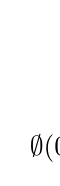
\begin{tikzpicture}[scale=0.8]
                \crd[right]{0}{0}{$\emptyset$}
                \crd[right]{0}{1}{$\s{(0,a)}$}
                \crd[right]{0}{2}{$\s{(0,a),(1,0,b)}$}
                \draw [ultra thick] (0,0) -- (0,1);
                \draw [ultra thick] (0,1) -- (0,2);
            \end{tikzpicture}
        \end{center}
    \end{example}
\end{frame}

\begin{frame}{Event Structure Semantics: Non-deterministic Choice}
    \begin{example}
        Let $a,b\in \mc{A}$ be some DyNetKAT actions and $a\oplus b$ a
        normal DyNetKAT term.
        $\mr{E} = \sem{a\oplus b}$ is an event structure
        $(E,\#,\vdash,L,l)$ where:
        \begin{align*}
            E & = \s{(0,a),(1,b)}                \\
              & (0,a) \# (1,b) , (1,b) \# (0,a)  \\
              & \e \vdash (0,a), \e \vdash (1,b) \\
            L & = \s{a,b}                        \\
              & l((0,a)) = a, l((1,b)) = b       
        \end{align*}
        The following diagram shows configurations of $\mr{E}$:
        \begin{center}
            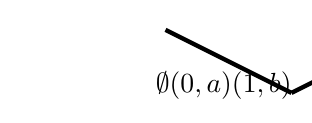
\begin{tikzpicture}[scale=0.8]
                \crd[above]{0}{0}{$\emptyset$}
                \crd[above]{-2}{1}{$\s{(0,a)}$}
                \crd[above]{2}{1}{$\s{(1,b)}$}
                \draw [ultra thick] (0,0) -- (-2,1);
                \draw [ultra thick] (0,0) -- (2,1);
            \end{tikzpicture}
        \end{center}
    \end{example}
\end{frame}

\begin{frame}{Event Structure Semantics: Parallel Composition}
    \begin{example}
        Let $a,b\in \mc{A}$ be some DyNetKAT actions and $a\parallel b$ a
        normal DyNetKAT term.
        $\mr{E} = \sem{a\parallel b}$ is an event structure
        $(E,\#,\vdash,L,l)$ where:
        \begin{align*}
            E  & = \s{(a,*),(*,b),(a,b)}                           \\
            \# & = \e                                              \\
               & \e \vdash (a,*), \e \vdash (*,b),\e \vdash (a,b)  \\
            L  & = \s{(a,*),(*,b),(a,b)}                           \\
               & l((a,*)) = (a,*), l((*,b)) = (*,b),l((a,b))=(a,b) 
        \end{align*}
    \end{example}
\end{frame}

\begin{frame}{Event Structure Semantics: Parallel Composition}
    \begin{example}
        The following diagram shows configurations of $\mr{E}$:
        \begin{center}
            \begin{tikzpicture}[scale=0.8]
                \crd[above]{0}{0}{$\emptyset$}
                \crd[left]{-2}{1}{$\s{(a,*)}$}
                \crd[right]{2}{1}{$\s{(*,b)}$}
                \crd[above]{0}{2}{$\s{(a,*),(*,b)}$}
                \crd[above]{2}{3}{$\s{(a,b)}$}
                \draw [ultra thick] (0,0) -- (-2,1);
                \draw [ultra thick] (0,0) -- (2,1);
                \draw [ultra thick] (2,1) -- (0,2);
                \draw [ultra thick] (-2,1) -- (0,2);
                \draw [ultra thick] (0,0) -- (2,3);
            \end{tikzpicture}
        \end{center}
    \end{example}
\end{frame}